% main.tex
\documentclass[11pt,a4paper]{ctexbook}
\usepackage{makeidx} % 调用 makeidx 宏包,用来处理索引
\usepackage{tabto}
\usepackage{tikz}                   % 绘制图形
\usepackage{tikz-3dplot}            % 绘制三维坐标系,坐标变换
\usepackage{siunitx}
\usepackage{indentfirst}
\usepackage{amsmath}
\usepackage{geometry}
\usepackage{pgfplots}
\usepackage{tcolorbox}
\usepackage{graphicx}
\usepackage{epstopdf}


\usepackage{tcolorbox}
\usepackage{colortbl}
\usepackage{geometry}


\usepackage{physics}
\usepackage{amsmath}
\usepackage{tikz}
\usepackage{mathdots}
\usepackage{yhmath}
\usepackage{cancel}
\usepackage{color}
\usepackage{siunitx}
\usepackage{array}
\usepackage{multirow}
\usepackage{amssymb}
\usepackage{gensymb}
\usepackage{tabularx}
\usepackage{extarrows}
\usepackage{booktabs}
\usetikzlibrary{fadings}
\usetikzlibrary{patterns}
\usetikzlibrary{shadows.blur}
\usetikzlibrary{shapes}


\usepackage{xparse}


\usepackage{newtxtext}
\usepackage{geometry}
\usepackage{lipsum} % 该宏包是通过 \lipsum 命令生成一段本文,正式使用时不需要引用该宏包
\usepackage[dvipsnames,svgnames]{xcolor}
\usepackage[strict]{changepage} % 提供一个 adjustwidth 环境
\usepackage{framed} % 实现方框效果

\def\TeacherName{郑振宇}


\usepackage{draftwatermark}         % 所有页加水印
%\usepackage[firstpage]{draftwatermark} % 只有第一页加水印
\SetWatermarkText{郑振宇}           % 设置水印内容
%\SetWatermarkText{\includegraphics{fig/texlion.png}}         % 设置水印logo
\SetWatermarkLightness{0.94}             % 设置水印透明度 0-1
\SetWatermarkScale{0.4}                   % 设置水印大小 0-1  
%

%--------------------------------------选择题---------------------------
\usepackage{ifthen}
\newlength{\la}
\newlength{\lb}
\newlength{\lc}
\newlength{\ld}
\newlength{\lhalf}
\newlength{\lquarter}
\newlength{\lmax}
\newcommand{\fourchoice}[4]{  
\settowidth{\la}{A.~#1~~~}  
\settowidth{\lb}{B.~#2~~~}  
\settowidth{\lc}{C.~#3~~~}  
\settowidth{\ld}{D.~#4~~~}  
\ifthenelse{\lengthtest{\la > \lb}}  
{\setlength{\lmax}{\la}}  
{\setlength{\lmax}{\lb}}  
\ifthenelse{\lengthtest{\lmax < \lc}}  
{\setlength{\lmax}{\lc}}  {}  
\ifthenelse{\lengthtest{\lmax < \ld}} 
{\setlength{\lmax}{\ld}}  {}  
\setlength{\lhalf}{0.5\linewidth}  
\setlength{\lquarter}{0.25\linewidth}  
\ifthenelse{\lengthtest{\lmax > \lhalf}} 
{\noindent{}A.~#1 \\ B.~#2 \\ C.~#3 \\ D.~#4 }  
{  \ifthenelse{\lengthtest{\lmax > \lquarter}}  
{\noindent\makebox[\lhalf][l]{A.~#1~~~}%    
\makebox[\lhalf][l]{B.~#2~~~}%    
\makebox[\lhalf][l]{C.~#3~~~}%    
\makebox[\lhalf][l]{D.~#4~~~}}%    
{\noindent\makebox[\lquarter][l]{A.~#1~~~}%      
\makebox[\lquarter][l]{B.~#2~~~}%      
\makebox[\lquarter][l]{C.~#3~~~}%      
\makebox[\lquarter][l]{D.~#4~~~}}}}
%-----------------------------------------------------------------------




% environment derived from framed.sty: see leftbar environment definition
\definecolor{formalshade}{rgb}{0.95,0.95,1} % 文本框颜色
% ------------------******-------------------
% 注意行末需要把空格注释掉,不然画出来的方框会有空白竖线
\newenvironment{formal}{%
\def\FrameCommand{%
\hspace{1pt}%
{\color{DarkBlue}\vrule width 2pt}%
{\color{formalshade}\vrule width 4pt}%
\colorbox{formalshade}%
}%
\MakeFramed{\advance\hsize-\width\FrameRestore}%
\noindent\hspace{-4.55pt}% disable indenting first paragraph
\begin{adjustwidth}{}{7pt}%
\vspace{2pt}\vspace{2pt}%
}
{%
\vspace{2pt}\end{adjustwidth}\endMakeFramed%
}
% ------------------******-------------------


\newcommand{\classinfo}[4]{
\begin{center}
    \begin{tabular}{ | m{5em}<{\centering} | m{4em}<{\centering}| m{4em}<{\centering} | m{4em}<{\centering} | m{5em}<{\centering} | m{5em}<{\centering} | m{4em}<{\centering} | m{5em}<{\centering} | } 
    \hline
    教师姓名& \TeacherName & 学生姓名&   & 等级& #1 & 上课时间 & \\ 
    \hline
    学\quad\quad 科& 高中数学 & 课题名称 &  \multicolumn{5}{c|}{#2} \\ 
    \hline
    教学目标 & \multicolumn{7}{l|}{#3} \\ 
    \hline
    教学重难点 & \multicolumn{7}{l|}{#4} \\ 
    \hline
    \end{tabular}
 \end{center}
}



\newif\ifprint

\newcommand{\xuanze}[1]{\ (
\ifprint
\ #1
\else
\hspace*{4em}
\fi)}

\newcommand{\tiankong}[1]{\ \underline{
\ifprint
\ #1
\else
\hspace*{5em}
\fi}}

\newif\ifjiexi
\NewDocumentEnvironment{jiexi}{ +b }{
\ifjiexi
\par
{\bfseries 解析}\, #1
\else
{\vspace{2cm}}
\fi
}{\par}

\newif\ifshowanswer
\showanswertrue %答案控制看这里

\ifshowanswer
\printtrue
\jiexitrue
\else
\printfalse
\jiexifalse
\fi 


\geometry{a4paper,hmargin=0.7in,vmargin=0.7in} %设置上下左右边距

\title{沪教版高中数学讲义} 
\author{ 郑振宇\thanks{邮箱:coyatzheng@gmail.com}}
\date{\today}


\begin{document}
\newtheorem{problem}{例}[section]
\newtheorem{hmwk}{}
\setlength{\parindent}{0em}


\maketitle



\chapter{集合与逻辑}
ssss
\chapter{等式和不等式}

\section{等式的性质与方程的解集}
\begin{enumerate}
    \item 等式的性质
    \begin{enumerate}
        \item 传递性 \NumTabs{16} 设$a,b$均为实数,如果$a=b$,且$b=c$,那么$a=c$ 
        \item 加法性质 \NumTabs{16} 设$a,b$均为实数,那么$a+c=b+c$ 
        \item 乘法性质 \NumTabs{16} 设$a,b$均为实数,那么$ac=bc$ 
    \end{enumerate}
    \item 方程的解集 \quad  含有未知数的等式称为方程.使得方程两端相等的未知数的值,称为方程的解或者方程的根。
    以方程的解为元素所构成的集合称为方程的解集。
\end{enumerate}

\section{一元二次方程的解集及根与系数的关系}

1、概念:形如 $ax^2+bx+c,(a \ne 0)$ 的方程为一元二次方程;\par
2、配方法:对一元二次方程进行配方得到方程:$\displaystyle(x + \frac{b}{2a})^2 = \frac{b^2-4ac}{4a^2} $ \par
3、判别式$\Delta$ \par
从配方之后的方程可以看出:原方程有没有解,取决于代数式$ b^2-4ac $的正负;基于$ b^2-4ac $的重要性,令称为该一元二次方程的判别式,它决定了一元二次方程解的个数问题;\par
(1)若$\Delta > 0$,原方程有两个不等的实数根,这两个根是$\displaystyle x_1 = \frac{-b+\sqrt{b^2-4ac}}{2a} , x_2 = \frac{-b-\sqrt{b^2-4ac}}{2a}$;\par
(2)若$\Delta = 0$,原方程有两个相等的实数根,$\displaystyle x_1 = x_2 = -\frac{b}{2a}$;\par
(3)若$\Delta < 0$,原方程没有实根;\par
4、韦达定理\par
当上述一元二次方程有实数解时,$\displaystyle x_1 = \frac{-b+\sqrt{b^2-4ac}}{2a} , x_2 = \frac{-b-\sqrt{b^2-4ac}}{2a}$ \par
则:$$ x_1+x_2=\frac{-b+\sqrt{\Delta}}{2a}+\frac{-b-\sqrt{\Delta}}{2a}=-\frac{b}{a}$$
$$ x_1 \cdot x_2=\frac{-b+\sqrt{b^2-4ac}}{2a} \cdot \frac{-b-\sqrt{b^2-4ac}}{2a}=  \frac{c}{a}$$

注意:在现在所学范围下,使用韦达定理时,需判别$\Delta = b^2-4ac \ge 0 $. \par
特别的:
$$x_1^2+x_2^2 = (x_1+x_2)^2-2x_1x_2 \qquad \qquad \frac{1}{x_1}+\frac{1}{x_2} = \frac{x_1+x_2}{x_1x_2}$$
$$(x_1-x_2)^2 = (x_1+x_2)^2-4x_1x_2 \qquad \qquad | x_1-x_2 | = \sqrt{(x_1+x_2)^2-4x_1x_2}$$
{一元二次方程的两根之差的绝对值$\displaystyle | x_1-x_2 | =  \frac{\sqrt{\Delta}}{|a|}$\par}


\clearpage
\section{第6课\quad 不等式的求解1}
\begin{formal}
    {\large \textbf{知识点一、一元一次不等式组求解}}
\end{formal}
(同大取大,同小取小,大小交叉中间找,大大小小没有解)

\begin{formal}
    {\large \textbf{知识点二、一元二次不等式求解}}
\end{formal}

(方程的根-函数草图-观察求解)

\begin{formal}
    {\large \textbf{知识点三、一元二次方程根的分布}}
\end{formal}

一元二次方程$ax^2+bx+c=0\quad (a,b,c \in R,a>0)$两实根为$x_1,x_2 \Leftrightarrow$函数$f(x)=ax^2+bx+c$与$x$轴交点为$(x_1,0),(x_2,0)$

(1)\quad $\displaystyle x_{1}>0,x_2>0 \Leftrightarrow \left\{
\begin{aligned}
\Delta \ge 0 \\
x_1+x_2>0 \\
x_1 \cdot x_2 > 0
\end{aligned}
\right. 
\Leftrightarrow 
\left\{
\begin{aligned}
\Delta \ge 0 \\
-\frac{b}{2a}>0 \\
f(0) > 0
\end{aligned}
\right. 
$   其中$\displaystyle \Delta=b^2-4ac,x_1+x_2=-\frac{b}{a},x_1 \cdot x_2=\frac{c}{a}$;\par

(2)\quad $\displaystyle x_{1}<0,x_2<0 \Leftrightarrow \left\{
\begin{aligned}
\Delta \ge 0 \\
x_1+x_2<0 \\
x_1 \cdot x_2 > 0
\end{aligned}
\right. 
\Leftrightarrow 
\left\{
\begin{aligned}
\Delta \ge 0 \\
-\frac{b}{2a}<0 \\
f(0) > 0
\end{aligned}
\right. 
$ ;\par
(3)\quad $\displaystyle x_{1}>0,x_2<0 \Leftrightarrow \left\{
\begin{aligned}
\Delta > 0 \\
x_1 \cdot x_2 < 0
\end{aligned}
\right. 
\Leftrightarrow 
f(0) < 0
$ ;\par
(4)\quad $\displaystyle x_{1}>m,x_2>m \Leftrightarrow \left\{
\begin{aligned}
\Delta \ge 0 \\
(x_1-m)+(x_2-m)>0 \\
(x_1-m)\cdot(x_2-m) > 0
\end{aligned}
\right. 
\Leftrightarrow 
\left\{
\begin{aligned}
\Delta \ge 0 \\
-\frac{b}{2a}>0 \\
f(m) > 0
\end{aligned} 
\right. 
$\par
(5)\quad $\displaystyle x_{1}<m<x_2 \Leftrightarrow \left\{
\begin{aligned}
\Delta > 0 \\
(x_1-m)\cdot(x_2-m) < 0
\end{aligned}
\right. 
\Leftrightarrow 
f(m) < 0
$\par
(6)\quad $\displaystyle x_{1},<x_2 \in(m,n) \Leftrightarrow \left\{
\begin{aligned}
\Delta \ge 0 \\
m<-\frac{b}{2a}<n \\
f(m) > 0\\
f(n) > 0
\end{aligned}
\right. 
$

\clearpage
\section{第7课\quad 不等式的求解2}

\begin{formal}
    {\large \textbf{知识点一、分式不等式的解法}}
\end{formal}

1、定义:型如$\displaystyle \frac{f(x)}{\varphi(x)}>0$或$\displaystyle \frac{f(x)}{\varphi(x)}<0$,(其中$f(x),\varphi(x)$为整式且$\varphi(x)\ne 0$)的不等式称为分式不等式.\par
2、解法\par
\begin{enumerate}
    \item 化分式不等式一边为零.
    \item 应用同号相乘(除)得正,异号相乘(除)得负,转化为同解不等式组解之
    \item 解分式不等式的基本思路是将其转化为整式不等式,在此过程中,变形的等价性尤为重要
    \item 分式不等式$\displaystyle \frac{ax+b}{cx+d}\ge 0(a,c \ne 0) \Leftrightarrow
    \left\{
        \begin{aligned}
        (ax+b)(cx+d)\ge 0 \\
        cx+d \ne 0 
        \end{aligned}
        \right. 
        (a,c \ne 0) 
    $\par
    $\displaystyle \frac{f(x)}{g(x)}> 0 \Leftrightarrow f(x)g(x)>0 $\par
    $\displaystyle \frac{f(x)}{g(x)}\ge 0 \Leftrightarrow f(x)g(x)>0
    \left\{
        \begin{aligned}
            f(x)g(x)\ge 0 \\
            g(x) \ne 0 
        \end{aligned}
        (a,c \ne 0)
        \right.  
    $\par

\end{enumerate}
\begin{formal}
    {\large \textbf{知识点二、一元高次不等式的解法--穿针引线 [补充内容]}}
\end{formal}

\begin{enumerate}
    \item 分解成若干个一次因式的积,并使每一个因式中最高次项的系数为正;
    \item 将每一个一次因式的根标在数轴上,从最大根的右上方依次通过每一点画曲线;并注意奇穿偶不穿;
    \item 根据曲线显现的符号变化规律,写出不等式的解集.\\ 
    例如$a_1<a_2<a_3<\cdots <a_n$,则不等式$(x-a_1)(x-a_2)\cdots(x-a_n)>0$或$(x-a_1)(x-a_2)\cdots(x-a_n)<0$的解法如下图(即“穿针引线”或“数轴标根法”):\par
    \begin{center}
    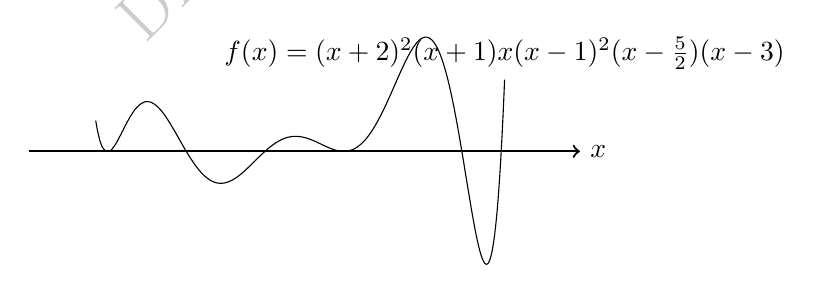
\begin{tikzpicture}
        % \draw[very thin,color=gray] (-0.1,-1.1) grid (3.9,8.1);
        \draw[->,thick] (-3,0) -- (4,0) node[right] {$x$}; 
        
        % \draw[domain=-6:6.5,samples=200] plot (\x,{sin((3*\x) r)});% node[right] {$f(x) = \sin x$};
        \draw[domain=-2.15:3.05,samples=500] plot (\x,{0.03*(\x+2)^2*(\x+1)*\x*(\x-1)^2*(\x-2.5)*(\x-3)}) node[above] {$f(x) = (x+2)^2(x+1)x(x-1)^2(x-\frac{5}{2})(x-3)$};
    \end{tikzpicture}
\end{center}

\end{enumerate}

\begin{formal}
    {\large \textbf{知识点三、含绝对值不等式的解法}}
\end{formal}

\begin{enumerate}
    \item 最简单的绝对值不等式的同解变形;
    $$
    |ax+b|<c \Leftrightarrow -c<ax+b<c 
    $$
    $$
    |ax+b|>c \Leftrightarrow ax+b<-c \text{\  或 \ }  ax+b>c
    $$
    \item 不等式$ |x|<a\ (a>0)$的解集就是求在数轴上到原点的距离小于$a$的点对应的实数$x$的集合.

\end{enumerate}
\clearpage
\section{第8课\quad 基本不等式及其应用}

\classinfo{C2}{2.3 基本不等式及其应用}{掌握基本不等式的基本应用方法以及解题逻辑;掌握三角形不等式的应用方法}{基本不等式}

\begin{formal}
    {\large \textbf{知识点一、平均值不等式}}
\end{formal}


\begin{enumerate}
    \item 对于正数$a,b$称$\displaystyle \frac{a+b}{2}\text{是}a,b\text{的算数平均值,并称}\sqrt{ab}\text{是}a,b\text{的几何平均值}$

    \item {\large{\textbf{平均值不等式:}}}\ 两个正数的算术平均值大于等于它们的几何平均值,即对于任意的正数,有
    $$
    \frac{a+b}{2}\ge \sqrt{ab},\ (a>0,b>0)
    $$
    当且仅当$a=b$是等号成立\\
    \\
    {\large{\textbf{三注意:}}}\\
    {\large{\textbf{“一正”:}}}不等式中的各项必须都是正数; \\
    {\large{\textbf{“二定”:}}}和定积最大,积定和最小; \\
    {\large{\textbf{“三相等”:}}}只有满足了不等式中等号成立的条件,才能使用基本不等式求最值.\\
    \item 平均值不等式的变式与推广
    \begin{enumerate}
        \item 加权平均$\ge$ 算术平均$\ge$ 几何平均:$\displaystyle \sqrt{\frac{a^2+b^2}{2}}\ge \frac{a+b}{2} \ge \sqrt{ab} , \ (a>0,b>0)$
    
        \item { 推广:$ a_1,a_2,a_3,\cdots,a_n$是$n$个正数,则$\displaystyle \frac{a_1,a_2,a_3,\cdots,a_n}{n}$称为这$n$个正数的算术平均数,\\ 
        $\sqrt[n]{a_1\cdot a_2\cdot a_3\cdot \cdots \cdot a_n}$称为这个正数的几何平均数,
        它们的关系是:
        $$\displaystyle \frac{a_1,a_2,a_3,\cdots,a_n}{n} \ge \sqrt[n]{a_1\cdot a_2\cdot a_3\cdot \cdots \cdot a_n}$$
        当且仅当$  a_1=a_2=a_3=\cdots=a_n$时等号成立。}
    \end{enumerate}
\end{enumerate}


\begin{tcolorbox} 
\centering
题型一:基本不等式基本应用
\end{tcolorbox}
\par
\begin{problem}
    设$x>0$,证明$\displaystyle x+\frac{1}{x} \ge 2$,并指出等号成立条件
    \begin{jiexi}
        因为$x>0$,有平均值不等式得:
        $$x+\frac{1}{x} \ge 2\sqrt{x\cdot\frac{1}{x}} = 2$$
        当$x=\frac{1}{x}$,即$x=1$时等号成立.
    \end{jiexi}
\end{problem}

\par
\begin{problem}
    证明:若$ a<0$,则$\displaystyle a+\frac{1}{a} \le -2$,并指出等号成立条件。
    \begin{jiexi}
       根据题意,$a<0$,则$-a>0$,左式$\displaystyle =a+\frac{1}{a}=-[(-a)+(-\frac{1}{a})]$,\\
       又由$\displaystyle (-a)+(-\frac{1}{a})\ge 2\sqrt{(-a)\cdot(-\frac{1}{a})} = 2$,则有$a+\frac{1}{a}\le -2$,当且仅当$a=-1$时,等号成立
    \end{jiexi}
\end{problem}

\par
\begin{problem}
    $x \ne 0,x\in R,$,则$\displaystyle =x+\frac{1}{x}$的取值范围\tiankong{$(-\infty,-2]\cup[2,+\infty)$}
\end{problem}

\par
\begin{problem}
    设$ab>0$,证明$\displaystyle \frac{b}{a}+\frac{a}{b}\ge 2$,并指出等号成立的条件
    \begin{jiexi}
        因为$ab>0$,所以$a,b$同号,因而$\displaystyle \frac{b}{a}>0,\frac{a}{b}>0$
        \\ 由平均值不等式,得
            $$
            \frac{b}{a}+\frac{a}{b}\ge 2\sqrt{\frac{b}{a}\cdot\frac{a}{b}}=2
            $$
            当且仅当$\displaystyle \frac{b}{a}=\frac{a}{b}$,即$a=b$时才成立.
     \end{jiexi}
\end{problem}

\par
\begin{problem}
    已知$a+b=1,a,b \in R$,求证:$\displaystyle a^2+b^2\ge \frac{1}{2}$,并指出等号成立的条件.
    \begin{jiexi}
        对任意的实数$a,b, \quad (a-b)^2 = a^2+b^2-2ab \ge 0\\$
        两边同时加上$a^2+b^2$得$\displaystyle 2(a^2+b^2)\ge 2ab +a^2+b^2=(a+b)^2\\
        a^2+b^2\ge \frac{(a+b)^2}{2} = \frac{1}{2}$.等号当且仅当$\displaystyle a=b=\frac{1}{2}$时成立.
    \end{jiexi}
\end{problem}

\par
\begin{problem}
    若对任意$a>0,b>0$,不等式$\displaystyle \frac{2}{a}+\frac{1}{b} \ge \frac{m}{2a+b}$恒成立,则$m$的取值范围是\tiankong{$(-\infty,9]$}
\end{problem}

\par
\begin{problem}
    设$x\in R$,函数$y=x(4-x)$的最大值\tiankong{4}
\end{problem}

\par
\begin{problem}
    设$a,b$为正数,且$a+2b=1$,比较$ab$与$\displaystyle \frac{1}{8}$的值的大小\tiankong{$\displaystyle ab < \frac{1}{8}$}
\end{problem}

\par
\begin{problem}
    已知$y=2x\sqrt{1-x^2}(0<x<1)$,求$y$的最大值\tiankong{1}
\end{problem}

\par
\begin{problem}
    若$x^2+y^2=1$,则$xy$的取值范围\tiankong{$\displaystyle [-\frac{1}{2},\frac{1}{2}]$}
\end{problem}

\par
\begin{problem}
    已知$\displaystyle a,b \in R^+,a^2+\frac{b^2}{2} = 1$,求$a\sqrt{1+b^2}$的最大值
    \begin{jiexi}
        $$\displaystyle a\sqrt{1+b^2}=\sqrt{2}\cdot(a\cdot \sqrt{\frac{1+b^2}{2}}) \le \sqrt{2}(\frac{a^2+\frac{1+b^2}{2}}{2}) = \sqrt{2}\cdot\frac{1}{2}=\frac{\sqrt{2}}{2}$$
        当且仅当$\displaystyle a=\sqrt{\frac{1+b^2}{2}}$时取等号,因此$a\sqrt{1+b^2}$得最大值为$\displaystyle \frac{\sqrt{2}}{2}$
    \end{jiexi}
\end{problem}

\par
\begin{problem}
    已知$a,b$均为正实数,求证:$\displaystyle \frac{2}{\frac{1}{a}+\frac{1}{b}}\le\sqrt{ab}\le\frac{a+b}{2}\le\sqrt{\frac{a^2+b^2}{2}}$,并指出等号成立的条件
    \begin{jiexi}
        $\displaystyle a>0,b>0\text{则}\frac{1}{a}>0,\frac{1}{b}>0,$由均值不等式得$\displaystyle \frac{\frac{1}{a}+\frac{1}{b}}{2}\ge\sqrt{\frac{1}{ab}}>0.\text{则}\frac{2}{\frac{1}{a}+\frac{1}{b}}\le\sqrt{ab} $,等号当且仅当$a=b$时成立.\\
        $(a-b)^2 = a^2+b^2-2ab \ge 0$
        两边同时加上$a^2+b^2$得$\displaystyle 2(a^2+b^2)\ge 2ab +a^2+b^2=(a+b)^2\\
        a^2+b^2\ge \frac{(a+b)^2}{2} $.等号当且仅当$\displaystyle a=b$时成立.\\
        由均值不等式得$\displaystyle \sqrt{ab}\le\frac{a+b}{2}$显然成立\\
        故$\displaystyle \frac{2}{\frac{1}{a}+\frac{1}{b}}\le\sqrt{ab}\le\frac{a+b}{2}\le\sqrt{\frac{a^2+b^2}{2}}$.等号当且仅当$\displaystyle a=b$时成立.
    \end{jiexi}
\end{problem}



\begin{tcolorbox} 
\centering
题型二:配凑法
\tcblower %增加了一条虚线
$$x+\frac{1}{x+a} \quad \Rightarrow \quad x+a+\frac{1}{x+a}-a$$
$$x(x-bx) \quad \Rightarrow \quad bx(a-bx)\cdot \frac{1}{b} $$
\end{tcolorbox}


\par
\begin{problem}
    函数$\displaystyle y=x+\frac{1}{x-1}$的最小值为\tiankong{3}
\end{problem}

\par
\begin{problem}
    已知$\displaystyle 0<x<\frac{1}{2}$,求$\displaystyle y=\frac{1}{2}x(1-2x)$的最大值为\tiankong{$\frac{1}{16}$}
\end{problem}

\par
\begin{problem}
    已知$\displaystyle x<\frac{5}{4}$,求函数$\displaystyle y=4x-2+\frac{1}{4x-5}$的最大值。
    \begin{jiexi}
        $\displaystyle x<\frac{5}{4},5-4x>0,y=4x-2+\frac{1}{4x-5}=-(5-4x+\frac{1}{5-4x})+3\le-2+3=1$,当且仅当$\displaystyle 5-4x=\frac{1}{5-4x}$,即$x=1$时等号成立,故$y_{max}=1$
    \end{jiexi}
\end{problem}

\par
\begin{problem}
    已知$\displaystyle x>\frac{3}{2},x+\frac{4}{2x-3}$的最小值为\tiankong{$\displaystyle 2\sqrt{2}+\frac{3}{2}$}
    \begin{jiexi}
        $\displaystyle x+\frac{4}{2x-3}=x+\frac{2}{x-\frac{3}{2}}=x-\frac{3}{2}+\frac{2}{x-\frac{3}{2}}+\frac{3}{2}\ge2\sqrt{2}+\frac{3}{2}$
    \end{jiexi}
\end{problem}

\begin{tcolorbox} 
    \centering
    题型三:换元法
    \tcblower %增加了一条虚线
    \begin{enumerate}
        \item 观察形式,型如$\displaystyle y=\frac{ex+f}{ax^2+bx+c}$或$\displaystyle y=\frac{ax^2+bx+c}{ex+f};(\frac{\text{一次}}{\text{二次}}\text{或}\frac{\text{二次}}{\text{一次}})$
        \item 令$t=ex+f$对式子进行配凑成$\displaystyle y=at+\frac{b}{t}$的形式,(对一次式进行整体换元)
        \item 再利用基本不等式求最值
    \end{enumerate}
\end{tcolorbox}


\par
\begin{problem}
    已知$x>0$,求函数$\displaystyle y=\frac{x^2+x+1}{x}$的最小值\tiankong{8}
\end{problem}

\par
\begin{problem}
    已知$x>-1$,求函数$\displaystyle y=\frac{x^2+x+1}{x+1}$的最小值\tiankong{1}
\end{problem}

\par
\begin{problem}
    已知$x>-2$,求函数$\displaystyle y=\frac{x+2}{x^2-x+6}$的最小值\tiankong{$\displaystyle \frac{4\sqrt{3}+5}{23}$}
\end{problem}

\par
\begin{problem}
    已知$x>-1$,求函数$\displaystyle y=\frac{x+1}{x^2+3x+3}$的最大值\tiankong{$\displaystyle \frac{1}{3}$}
\end{problem}

\par
\begin{problem}
    函数$\displaystyle y=\frac{6\sqrt{x^2+2}}{x^2+4}$的最大值为\tiankong{$\displaystyle \frac{3\sqrt{2}}{2}$}
\end{problem}


\begin{tcolorbox} 
    \centering
    题型四:“1”的代换(齐次化)
    \tcblower %增加了一条虚线
    题目已知$x+y=m$,求$\displaystyle \frac{a}{x}+\frac{b}{y}$\quad 或\quad 已知$\displaystyle \frac{a}{x}+\frac{b}{y}=m$,求$x+y$时\\
    (1)把已知条件变成“1” \\
    (2)两式乘起来,用基本不等式
\end{tcolorbox}

\par
\begin{problem}
    设$a>0,b>0$且$a+b=2$,则$\displaystyle \frac{1}{a}+\frac{1}{b}$的最小值为\tiankong{2}
\end{problem}

\par
\begin{problem}
    设$a>0,b>0$且$\displaystyle \frac{3}{a}+\frac{4}{b}=1$,则$a+b$的最小值为\tiankong{$4\sqrt{3}+7$}
\end{problem}

\par
\begin{problem}
    设$a>0,b>0$且$a+b=2$,则$\displaystyle \frac{1}{a}+\frac{1}{b-1}$的最小值为\tiankong{4}
\end{problem}

\par
\begin{problem}
    若$x,y$为正实数满足$x+3y=5xy$,求$3x+4y$的最小值\tiankong{5}
\end{problem}

\par
\begin{problem}
    设$a>0,b>0$,则$\displaystyle \frac{1}{a+1}+\frac{1}{b+1}=1$,则$a+2b$的最小值为\tiankong{5}
\end{problem}

\par
\begin{problem}
    设$x>0,y>0$,且$x+y=1,$则$\displaystyle \frac{1}{2x+y}+\frac{2}{y+3}$的最小值为\tiankong{$\displaystyle \frac{3+2\sqrt{2}}{5}$}
\end{problem}

\par
\begin{problem}
    设$x>0,y>0$,且$2x+3y=5,$则$\displaystyle \frac{1}{x+y}+\frac{2}{y+3}$的最小值为\tiankong{1}
\end{problem}

\par
\begin{problem}
    设$A,B,C$为$\bigtriangleup ABC$的三个内角,则$\displaystyle \frac{4}{A}+\frac{1}{B+C}$的最小值为\tiankong{$\displaystyle \frac{9}{\pi}$}
\end{problem}

\par
\begin{problem}
    设$a,b$是正实数,且$a+2b=2$,则$\displaystyle \frac{a^2}{a+1}+\frac{4b^2}{2b+1}$的最小值是\tiankong{1}
    \begin{jiexi}
        $\displaystyle \frac{a^2}{a+1}+\frac{4b^2}{2b+1}=\frac{1}{4}(\frac{a^2}{a+1}+\frac{4b^2}{2b+1})\cdot(a+1+2b+1)=
        \frac{1}{4}[a^2+4b^2+\frac{a^2(2b+1)}{a+1}+\frac{4b^2(a+1)}{2b+1}]\ge\frac{1}{4}(a^2+4b^2+4ab)=\frac{1}{4}(a+2b)^2=1$,当且仅当$a(2b+1)=2b(a+1)$时取等号.
    \end{jiexi}
\end{problem}

\par
\begin{problem}
    设$a+b=2019,b>0$,则当$a=$\tiankong{$\displaystyle -\frac{2019}{2018}$}时,$\displaystyle \frac{1}{2019|a|}+\frac{|a|}{b}$取的最小值
\end{problem}

\par
\begin{problem}
    非零实数$x,y,z$满足$x^2+y^2+z^2=1$,则$\displaystyle \frac{1}{x^2}+\frac{1}{y^2}+\frac{1}{z^2}$的最小值是\tiankong{9}
\end{problem}

\par
\begin{problem}
    若正数$a,b$满足$\displaystyle \frac{1}{a}+\frac{1}{b}=1,\frac{1}{a-1}+\frac{9}{b-1}$,的最小值为\tiankong{6}
\end{problem}



\begin{tcolorbox} 
    \centering
    题型五:消元法
    \tcblower %增加了一条虚线
    (1)写:根据问题形式写出基本不等式\\
    (2)换:求谁留谁,把另一个通过条件整体替换掉\\
    (3)解:将$ab$或$a+b$视作整体,解二次不等式
\end{tcolorbox}

\par
\begin{problem}
    设$a,b$为正实数,且$ab=a+b+3$,则求$ab$和$a+b$的取值范围\tiankong{$[9,+\infty)$}和\tiankong{$[6,+\infty)$}
\end{problem}

\par
\begin{problem}
    设$x,y$为正实数,且$x+2y+2xy=8$,则求$x+2y$的最小值\tiankong{8}
\end{problem}

\par
\begin{problem}
    设$x,y$为正实数,且$2x+3y+xy=6$,则求$2xy$的最小值\tiankong{0}
\end{problem}

\par
\begin{problem}
    已知$a>0,b>0,$当$\displaystyle (a+4b)^2+\frac{1}{ab}$取到最小值时,$b=$\tiankong{$\displaystyle \frac{1}{4}$}
    \begin{jiexi}
        $\displaystyle (a+4b)^2+\frac{1}{ab}\ge(2\sqrt{a\cdot4b})^2+\frac{1}{ab}=16ab+\frac{1}{ab}\ge 2\sqrt{16}=8$.
    \end{jiexi}
\end{problem}

\par
\begin{problem}
    设$a>b>0$,求$\displaystyle a^2+\frac{16}{b(a-b)}$的最小值\tiankong{16}
    \begin{jiexi}
        $\displaystyle a^2+\frac{16}{b(a-b)}\ge a^2+\frac{16}{[\frac{b+(a-b)}{2}]^2}=a^2+\frac{64}{a^2}\ge16$.
    \end{jiexi}
\end{problem}

\par
\begin{problem}
    当$0<x<a$时,不等式$\displaystyle \frac{1}{x^2}+\frac{1}{(a-x)^2}\ge2$恒成立,求$a$的最大值
    \begin{jiexi}
        $\displaystyle \frac{1}{x^2}+\frac{1}{(a-x)^2}\ge 2\sqrt{\frac{1}{x^2(a-x)^2}}=\frac{2}{x(a-x)}\ge \frac{2}{\frac{[x+(a-x)]^2}{4}}=\frac{8}{a^2}$.当且仅当$x=\frac{a}{2}$时,取得最小值.所以$\displaystyle \frac{8}{a^2}\ge2,\text{则}a\le2$,故实数$a$的最大值为2
    \end{jiexi}
\end{problem}




\begin{tcolorbox} 
    \centering
    题型六:基本不等式的应用
\end{tcolorbox}

\par
\begin{problem}
    在城市旧城改造中,某小区为了升级居住环境,拟在小区的闲置地中规划一个面积为$200m^2$的矩形区域(如图所示),按规划要求:在矩形内的四周安排$2m$宽的绿化,绿化造价为200元/$m^2$,中间区域地面硬化以方便后期放置各类健身器材,硬化造价为100元/$m^2$.设矩形的长为$x(m)$.\\
    \includegraphics[scale=1.0]{pictures/image1.png}\\
    (1)设总造价$y$(元)表示为长度$x(m)$的函数;\\
    (2)当$x(m)$取何值时,总造价最低,并求出最低总造价.\\
    \begin{jiexi}
        (1)由矩形的长为$x$,则矩形的宽为$\displaystyle \frac{200}{x}$,
则中间区域的长为$x-4$,宽为$\displaystyle \frac{200}{x}-4$,则定义域为$x\in(4,50)$,
则$\displaystyle y=100\times[(x-4)(\frac{200}{x}-4)]+200[200-(x-4)(\frac{200}{x}-4)]$,
整理得$\displaystyle y=18400+400(x+\frac{200}{x}),x\in(4,50)$.\\
(2)$\displaystyle x+\frac{200}{x}\ge 2\sqrt{x\cdot\frac{200}{x}}=20\sqrt{2}$,当且仅当$\displaystyle x=\frac{200}{x}$时取等号,即$x=10\sqrt{2}\in (4,50)$,
所以当$x=10\sqrt{2}$时,总造价最低为$18400+8000\sqrt{2}$元.
    \end{jiexi}
\end{problem}



\par
\begin{problem}
    在面积为$\pi$的圆中作一个内接矩形,使它的面积最大.求此矩形面积的最大值及此时矩形的各边长.
    \begin{jiexi}
        $2,\sqrt{2},\sqrt{2}$
    \end{jiexi}
\end{problem}


\begin{tcolorbox} 
    \centering
题型七:综合题
\end{tcolorbox}

\par
\begin{problem}
    设实数$x,y$满足$2x+y=1$.
    \begin{enumerate}
        \item 求$4x2+y2+3xy$的最小值
        \item 若$x>0,y>0$,求$\displaystyle \frac{1}{x}+\frac{2}{y}-\sqrt{2xy}$的最小值
    \end{enumerate}
    \begin{jiexi}
        (I)因为$2x+y=1$,则$y=1﹣2x$,
所以$4x^2+y^2+3xy=4x^2+(1﹣2x)^2+3x(1﹣2x)=4x2+1+4x2﹣4x+3x﹣6x2=2x2﹣x+1$,
当$x=\frac{1}{4}$时,$\displaystyle 2(x-\frac{1}{4})^2+\frac{7}{8}$取得最小值,最小值为$\frac{7}{8}$,
所以当$\displaystyle x=\frac{1}{4},y=\frac{1}{2}$时,$4x^2+y^2+3xy$ 取得最小值$\displaystyle \frac{7}{8}$.\\
(II)因为$x>0,y<0,2x+y=1,$
所以$\displaystyle (\frac{1}{x}+\frac{2}{y})=(\frac{1}{x}+\frac{2}{y})(2x+y)=4+\frac{y}{x}+\frac{4x}{y}\ge4+2\sqrt{\frac{y}{x}\cdot\frac{4x}{y}}=4$,
当且仅当 $\displaystyle \frac{y}{x}=\frac{4x}{y}$,即$\displaystyle 2x=y=\frac{1}{2}$ 时取等号,
又因为$2x+y\ge2\sqrt{2x\cdot y}=2\sqrt{2xy}$,
所以$\displaystyle -\sqrt{2xy}\ge -\frac{2x+y}{2}=-\frac{1}{2}$,当且仅当$\displaystyle 2x=y=\frac{1}{2}$ 时等号成立,
所以$\displaystyle \frac{1}{2}+\frac{2}{y}-\sqrt{2xy}\ge8-\frac{1}{2}=\frac{15}{2}$,当且仅当$2x=y=\frac{1}{2}$ 时等号成立,
所以$\displaystyle \frac{1}{x}+\frac{2}{y}-\sqrt{2xy}$ 的最小值为$\displaystyle \frac{15}{2}$.
    \end{jiexi}
\end{problem}

\par
\begin{problem}
    若实数$x、y、m$满足$|x-m|<|y-m|$,则称x比y更接近m.
    \begin{enumerate}
        \item 若4比$x^2-3x$更接近0,求x的取值范围
        \item 对任意两个不相等的正数a、b,判断并证明:$(a+b)$和$\displaystyle (\frac{b^2}{a^2}+\frac{a^2}{b^2})$哪个更接近$2\sqrt{ab}$
    \end{enumerate}
    \begin{jiexi}
        \includegraphics[scale=1.3]{pictures/image2.png}\\
    \end{jiexi}
\end{problem}

\begin{formal}
    {\large \textbf{知识点二、三角不等式}}
\end{formal}
三角不等式:两个实数和的绝对值小于等于他们绝对值的和,
即对于任意给定的实数$a,b$,有$$|a+b|\le|a|+|b|$$且等号当且仅当$ab\ge0$时成立\\
如果$a,b$是实数,那么

\begin{enumerate}
    \item $||a|-|b||\le|a+b|\le |a|+|b|$且左等号当且仅当$ab\le0$时成立;且右等号当且仅当$ab\ge0$时成立
    \item $||a|-|b||\le|a-b|\le |a|+|b|$且左等号当且仅当$ab\ge0$时成立;且右等号当且仅当$ab\le0$时成立
\end{enumerate}

推论:$|a_1+a_2+\cdots+a_n|\le |a_1|+|a_2|+\cdots+|a_n|$,当且仅当$ab\ge0$时成立


\begin{tcolorbox} 
    \centering
    综合题
    \tcblower %增加了一条虚线
    使用三角不等式或者前面学的绝对值不等式解题
\end{tcolorbox}


\par
\begin{problem}
    \begin{enumerate}
        \item 写出不等式$|x+y|\le|x|+|y|$等号成立的一个充要条件是\tiankong{$xy\ge0\text{或}x=ky,k>0$},\\
        一个充分非必要条件是\tiankong{$x=0$},\\
        一个必要非充分条件是\tiankong{$xy\ge-1$};
        \item 写出不等式$|x|-|y|\le|x-y|$等号成立的一个充要条件是\tiankong{$xy\ge y^2$}
        \item 写出不等式$|x|-|y|\le|x+y|$等号成立的一个充要条件是\tiankong{$xy+y^2\le 0$}
        \item 写出不等式$|x-y|\le|x|+|y|$等号成立的一个充要条件是\tiankong{$xy\le 0$}
    \end{enumerate}
\end{problem}

\par
\begin{problem}
    代数式$y=|x-4|+|x-6|$的最小值为\tiankong{2}
\end{problem}

\par
\begin{problem}
    已知 $\displaystyle |x|<\frac{a}{4},|y|<\frac{a}{6}.$求证:$|2x-3y|<a$
\end{problem}

\par
\begin{problem}
    已知 $\displaystyle |x-a|<\frac{c}{2},|y-b|<\frac{c}{2}$,求证$|(x+y)-(a+b)|<c$ 
\end{problem}

\par
\begin{problem}
    $x$为实数,且$|x-5|+|x-3|<m$有解,则$m$的取值范围是\tiankong{$(2,+\infty)$}
\end{problem}

\par
\begin{problem}
    不等式$|x-a|+|x-3|>4$对一切实数x恒成立,求实数a的取值范围\tiankong{$(-\infty,-1)\cup(7,+\infty)$}
\end{problem}

\par
\begin{problem}
    若关于x的不等式$|x-1|+|ax-1|\ge2x$对于任意$x>0$恒成立,则实数a的取值范围是\tiankong{$(-\infty,-1]\cup[3,+\infty)$} 
\end{problem}

\par
\begin{problem}
    若对任意$a\in(1,+\infty)$,存在实数$x$,使得$\displaystyle |x-a|-|x+\frac{1}{a-1}|+x^2+a^2\le 2ax+a+m$成立,则实数$m$的最小值是\tiankong{$-2-2\sqrt{2}$}
    \begin{jiexi}
        对任意$a\in(1,+\infty)$,存在实数$x$,使得$\displaystyle |x-a|-|x+\frac{1}{a-1}|+(x-a)^2\le a+m$成立,
因为$\displaystyle |x-a|-|x+\frac{1}{a-1}|+(x-a)^2\ge -|a+\frac{1}{a-1}|$,当且仅当$x=a$时等号成立,
所以有$-|a+\frac{1}{a-1}|$对任意$a\in(1,+\infty)$恒成立,
即$\displaystyle -m\le 2a+\frac{1}{a-1}=2(a-1)+\frac{1}{a-1}+2$对任意$a\in(1,+\infty)$恒成立,
由于$\displaystyle 2(a-1)+\frac{1}{a-1}+2\ge 2\sqrt{2}+2$,当且仅当$\displaystyle 2(a-1)=\frac{1}{a-1}$,即$\displaystyle a=\frac{\sqrt{2}}{2}+1$时等号成立;
所以$-m\le2\sqrt{2}+2$,即$m\ge -2\sqrt{2}-2$.所以实数m的最小值是$-2\sqrt{2}-2$
    \end{jiexi}
\end{problem}

\clearpage
\textbf{【课后作业】}\\
\textbf{一、填空题:本大题共12小题,每小题5分,共60分.把答案填在答题卡中的横线上}

\begin{hmwk}
    (2010·湖北·一模)当$x>1$时,$\displaystyle x+\frac{4}{x-1}$的最小值为\tiankong{5}
\end{hmwk}

\begin{hmwk}
    (22-23高一上·湖北武汉·期中)若实数$x>1,y>1,$且$x+2y=5$,则$\displaystyle \frac{1}{x-1}+\frac{1}{y-1}$的最小值为\tiankong{$\displaystyle \frac{3}{2}+\sqrt{2}$}
\end{hmwk}

\begin{hmwk}
    (2023·山西大同·模拟预测)已知$\displaystyle a>0,b>0,a\ge \frac{1}{a}+\frac{2}{b},b \ge \frac{1}{b}+\frac{2}{a}$,则$a+b$的最小值为\tiankong{$2\sqrt{3}$}
    \begin{jiexi}
    $\displaystyle a+b \ge \frac{3}{a}+\frac{3}{b}$,又$a>0,b>0,$
    所以$\displaystyle (a+b)^2 \ge (\frac{3}{a}+\frac{3}{b})(a+b)=6+\frac{3b}{a}+\frac{3a}{b}\ge 12$,当且仅当$a=b=\sqrt{3}$时取等号.
    所以$a+b\ge2\sqrt{3}$,当且仅当$a=b=\sqrt{3}$时取等号.
    \end{jiexi}
\end{hmwk}

\begin{hmwk}
    (23-24高一上·广东河源·阶段练习)若正数$x,y$满足$\displaystyle \frac{1}{x}+\frac{8}{y}=1$,则$x+2y$的最小值为\tiankong{25}
\end{hmwk}

\begin{hmwk}
    (23-24高一下·河北·期末)已知$a>0,b>0$,且$9a+b=ab$,则$a+4b$的最小值为\tiankong{49}
\end{hmwk}

\begin{hmwk}
    (23-24高一下·云南曲靖·阶段练习)已知$x>0,y>0$,且$x+y=3$,则$\displaystyle \frac{y}{x+1}+\frac{1}{y}$的最小值为\tiankong{$\frac{5}{4}$}
\end{hmwk}

\begin{hmwk}
    (24-25高一上·全国·课前预习)若不等式$\displaystyle \frac{x}{x^2+3x+1}\le a$对一切正实数x都成立,则实数a的取值范围是\tiankong{$[\frac{1}{5},+\infty)$}
\end{hmwk}

\begin{hmwk}
    (23-24高二下·浙江绍兴·期中)已知$a>0,b>0$,且$a+2b=1$,则$\displaystyle \frac{1}{b}+\frac{8}{a+b}$的最小值为\tiankong{$9+4\sqrt{2}$}
\end{hmwk}

\end{document}